\documentclass[twoside]{article}
\usepackage[UTF8]{ctex} 
\usepackage{geometry}
 \geometry{
 a4paper,
 total={170mm,257mm},
 left=14.5mm,
 top=26mm,
 bottom=22mm,
 right=14.5mm
 }
 \usepackage{graphicx}
 \usepackage{titling}
\usepackage{ifthen}
 \title{Transformer中Self-Attention的快速计算}
\author{刘明道\ 滕嘉彦}

\usepackage{fancyhdr}
\usepackage[normalem]{ulem}
\usepackage{cmbright}
\usepackage{titlesec}
\usepackage{sectsty}
\usepackage{xstring}

\pagestyle{fancy}
\fancyhf{}
\fancyhead[RO]{
    \ifthenelse{\equal{\thepage}{1}}{
    }{
    \rule[0.66\baselineskip]{0.31\textwidth}{0.4pt}\hspace{0.02\textwidth}
    
    \vspace{-30pt}
    \thepage
    }
}

\fancyhead[LO]{
    \ifthenelse{\equal{\thepage}{1}}{
        \songti \zihao{-5}“数值分析”期末项目总结报告(2023 年春季学期)
        \vskip 2pt
        \hrule width0.9\headwidth\vskip1pt\hrule width0.9\headwidth
    }{\
    \heiti \zihao{-5}
    \theauthor :\thetitle
    }
}
\fancyhead[LE]{
\hspace{0.02\textwidth}\rule[0.65\baselineskip]{0.63\textwidth}{0.4pt}

\vspace{-30pt}
\thepage
}

% 设置页眉线的位置和粗细
\renewcommand{\headrulewidth}{0pt} % 去除默认的页眉线
\renewcommand{\footrulewidth}{0pt} % 去除默认的页脚线

% defs 
\newcommand{\printtitle}[1]{
    \vspace{10pt}
    \noindent{\heiti\zihao{3} #1}
}
\newcommand{\printauthor}[1]{
    \vspace{6pt}
    \noindent{\fangsong\zihao{4}\scalebox{0.66}[1] #1}
    \vspace{6pt}
}
\newcommand{\printcontact}[1]{{\songti\fontsize{10pt}{12pt}\selectfont\raggedright #1}}
\newcommand{\intro}[2]{
  \vspace{0.5\baselineskip}
  \noindent
  {\heiti \zihao{5} #1}
  {\songti \zihao{5} #2}
  \vspace{0.2\baselineskip}
}

% section
\titleformat{\section}[hang]{\normalfont\raggedright}{{\heiti\zihao{4} \thesection}}{1em}{} % 居左对齐
\titlespacing{\section}{0pt}{3pt}{4pt} 

% subsection
\titleformat{\subsection}{\normalfont\heiti\zihao{4}}{\thesubsection}{1em}{}
\titlespacing{\subsection}{0pt}{0.15\baselineskip}{0.15\baselineskip}

\usepackage{indentfirst} 
\setlength{\parindent}{2em} % 首行缩进2字符
\usepackage{setspace} 
\singlespacing % 单倍行距

\newcommand{\s}[1]{\section{\normalfont #1}}
\newcommand{\subs}[1]{\subsection{\normalfont #1}}
\newcommand{\subsubs}[1]{\subsubsection{\normalfont #1}}

% reference
\usepackage[style=ieee]{biblatex}
\addbibresource{references.bib}
\defbibheading{refheading}[参考文献]{%
  \section*{#1}% 以 \section 格式打印章节标题
}

% copy from mega
\usepackage{hyperref}       % hyperlinks
\hypersetup{
    colorlinks=true,
    linkcolor=blue,
    citecolor=blue,
    urlcolor=blue,
}
\usepackage{enumitem}
\usepackage{bm}
\usepackage{url}            % simple URL typesetting
\usepackage{wrapfig,lipsum,booktabs}       % professional-quality tables
\usepackage{amsfonts}       % blackboard math symbols
\usepackage{nicefrac}       % compact symbols for 1/2, etc.
\usepackage{fontspec}
\usepackage{microtype}      % microtypography
%\usepackage{todonotes}      % [disable]

\usepackage{caption}
\usepackage{subcaption}

\usepackage{amssymb}
% \usepackage[ruled,lined]{algorithm2e}
\usepackage{algorithm}
\usepackage{algorithmicx}
\usepackage{framed,graphicx}
%\usepackage[lofdepth,lotdepth]{subfig}
\usepackage{amsthm}
\usepackage{xcolor}
\usepackage{amsmath}
\usepackage{bigints}
% For Tables
\usepackage{multirow}
\usepackage{pifont}
\usepackage{xspace}
%\usepackage{arydshln}

\theoremstyle{plain}
\newcounter{theoremcounter}
\newtheorem{theorem}[theoremcounter]{定理}
\newtheorem{lemma}[theoremcounter]{引理}
\newtheorem{corollary}{推论}[theoremcounter]
\newcommand{\op}{\mathsf{op}}

%\theoremstyle{definition}
%\newcounter{definitioncounter}
%\newtheorem{definition}[definitioncounter]{Definition}
\newcommand{\xmark}{\ding{55}\xspace}%
\newcommand{\argmax}{\operatornamewithlimits{argmax}}
\newcommand{\argmin}{\operatornamewithlimits{argmin}}
%\newcommand{\inf}{\operatornamewithlimits{inf}}
%\newcommand{\sup}{\operatornamewithlimits{sup}}

\newcommand{\FIXME}[1]{\textcolor{red}{[#1]}}
\newcommand{\gn}[1]{\textcolor{magenta}{\bf\small [#1 --GN]}}
\newcommand{\xk}[1]{\textcolor{green}{\bf\small [#1 --XK]}}
\newcommand{\cz}[1]{\textcolor{orange}{\bf\small [#1 --CZ]}}
\newcommand{\jh}[1]{\textcolor{brown}{\bf\small [#1 --JH]}}

% % copy fromm skyformer
% \usepackage{hyperref}    % hyperlinks
% \usepackage{url}            % simple URL typesetting
% \usepackage{booktabs}       % professional-quality tables
% \usepackage{amsfonts}       % blackboard math symbols
% \usepackage{nicefrac}       % compact symbols for 1/2, etc.
% \usepackage{microtype}      % microtypography

% \usepackage[table,dvipsnames]{xcolor}
% \usepackage{url}


\renewcommand*{\ttdefault}{cmtt}
\usepackage{graphicx}               % Include graph
\usepackage{tabularx}               % Better table formatting
\newcolumntype{C}{>{\centering\arraybackslash}X}
\usepackage{multirow}               % Multi-row in tables
\usepackage{diagbox}                % Diagonal line in tables
\usepackage{hhline}                 % Draw double line in tables
\usepackage{color}                  % Text and background color
\usepackage{amsmath}                % Formula
\usepackage{amssymb}                % Formula
\usepackage{mathtools}              % Formula
\usepackage{enumitem}               % Better itemize environment
\usepackage{verbatim}               % comment env
\usepackage{multirow}
\newcommand{\bs}{\boldsymbol}
\newcommand{\ola}{\overleftarrow}
\newcommand{\ora}{\overrightarrow}
\newcommand{\ccgreen}{\cellcolor{Emerald!10}}
\newcommand{\ccdgreen}{\cellcolor{Emerald!20}}
\newcommand{\ccddgreen}{\cellcolor{Emerald!35}}
\newcommand{\x}{\checkmark}


\newtheorem{definition}{Definition} % definition in amsmath
\usepackage{ulem} % for delete line

\usepackage{bigstrut}

\begin{document}

\printtitle{\thetitle}

\printauthor{\theauthor}

\printcontact{(计算机系,学号:2020011156,2020011109,手机号:18747201120,18801384297)}

\songti\zihao{5}

\intro{摘\quad 要:}{Transformer 模型有很强的长序列建模能力,但Self-Attention操作对序列长度的平方时间复杂度限制了 Transformer 模型对长序列的处理速度。我们将讨论4种针对 Self-Attention 机制的加速方法,分别是Cosformer,LARA,Skyformer和 MEGA。实验部分,我们在 Long Range Arena~\cite{tay2021long} 基准上验证了以上方法的长序列建模能力,探索了方法中参数的作用效果,测量了不同方法在训练和推理过程中的加速效果,并将其进行对比,讨论不同算法的优势和劣势。我们将实验的代码开源于 \url{https://github.com/Btlmd/AttentionAccelerations}。}

\intro{关键词:}{Self-Attention机制;计算加速}
\vspace{-10pt}

\s{引言} 
    Transformer模型~\cite{vaswani2017attention}是用于序列建模的强大神经网络。它们已成功应用于各个领域,例如自然语言处理、计算机视觉、生物信息学等。 Transformer 模型的核心构建块是注意力机制,它捕获序列元素之间的复杂交互。与传统的循环神经网络(RNN)和卷积神经网络(CNN)相比,基于Transformer的架构在数据规模上通常更具可扩展性~\cite{brown2020language},且在获取全局信息方面具有较弱的归纳偏差,因此在许多任务上表现出色。

点积注意力机制和softmax归一化是Transformer捕捉长距离依赖关系的基石。
然而,它在序列长度方面的二次空间和时间复杂度使得它的计算开销非常高,特别是对于较长的输入。这使得Transformer 无法在资源有限的情况下支持长序列处理和大批量。

\hspace{0.2cm}

为了解决这个问题,最近出现了许多提高计算效率的高效 Transformer模型。

一类工作侧重于注意力矩阵的稀疏化,它通过将自注意力限制在预定义稀疏模式指定的位置来提高 Transformer 的效率。但是,当重要的标记相关性在多跳之外时,与全注意力相比,利用稀疏性可能会牺牲模型表达能力。

另一类工作通过通过在注意力结构上引入低秩假设,对$n\times n$矩阵乘法进行近似,第一行工作避免通过各种近似值显式计算 n × n 矩阵,例如通过核化的点积计算~\cite{wang2020linformer}或随机投影~\cite{peng2021random}。~\cite{choromanski2020rethinking} 指出softmax结构与高斯核密切相关,差别仅为对角矩阵的乘法,因为当展开平方的欧氏距离时,成对的点积自然出现。Self-Attention和高斯核之间联系紧密,高斯核的形式可将注意力分配给不同的元素。与softmax函数相比,高斯核可以自动执行与softmax相同的归一化操作。

\hspace{0.2cm}

然而,由于对Self-Attention的近似存在很大挑战,所以上述改进的计算效率常会牺牲模型的表达能力。更严重的是,许多近似算法引入了额外注意力矩阵假设,如经典的Linfomer~\cite{wang2020linformer} 或仅对softmax操作进行的近似只在固定范围内成立~\cite{choromanski2020rethinking} 。

为了进一步探索不同方法对于Self-Attention的计算效率和表现性能的影响,我们在本学期的“数值分析”课程项目中对Cosformer~\cite{zhen2022cosformer},LARA\cite{pmlr-v162-zheng22b},Skyformer~\cite{chen2021skyformer} 和 MEGA~\cite{ma2023mega} 这四种Self-Attention 的快速计算模型进行了复现,并实际测量了其长序列建模表现,以及在训练和推理过程中的性能。

\hspace{0.2cm}

Cosformer 是一种线性Transformer的新变体, 它基于 softmax attention 的两个关键属性:一是注意力矩阵的非负性,二是可以集中注意力矩阵的分布的非线性重加权方案。作为其线性替代品,Cosformer 通过线性运算符和基于余弦的距离重新加权机制来满足这些属性。
具体来说,它通过在计算相似性分数之前将特征传递给 ReLU 激活函数来强制执行非负属性。通过这种方式,它鼓励模型避免聚合负相关的上下文信息。此外,它采用 cos 重新加权方案来稳定注意力权重。这有助于模型放大局部相关性,这些相关性通常包含更多与自然语言任务相关的信息。由于托勒密定理,Cosformer的注意力可以精确地分解为线性形式,
它可以在随意和交叉注意中实现与普通Transformer相当或更好的精度。

\hspace{0.2cm}

LARA(线性随机注意力)是随机特征注意力(RFA)\cite{peng2021random}和随机注意力(RA)的结合。其中RFA通过将指数核线性化为随机特征图的点积来近似 softmax 注意力,尽管实现了线性时间和空间复杂度,但整体上是有偏估计。RA通过每个查询独有的分布构造正随机特征,可以对查询特定信息进行更细粒度的处理,并大大提高近似保真度,是softmax的无偏估计,但具有二次复杂度。LARA应用多重重要性采样 \cite{veach1995optimally} 来概括 RFA 的重要性抽样公式,针对不同的查询自适应地近似 softmax 注意力,保留 RA 的查询特定属性。同时,由于这些建议在所有查询之间共享,它继承了 RFA 中有效的计算重用并实现了线性复杂度。

\hspace{0.2cm}

Skyformer将\textit{nystrom}方法\cite{williams2001using, drineas2005nystrom}应用于非半正定的经验高斯核矩阵(一般情况下查询矩阵不等于键矩阵),
具体实现方式是将核化注意力得分矩阵提升为一个大型半正定矩阵,其中包含未归一化的注意力得分矩阵作为非对角块。
Skyformer在核化注意力的谱范数下具有较小的矩阵近似误差,且显著能加速计算。

\hspace{0.2cm}

MEGA(门控移动平均注意力)是一种配备移动平均线的门控注意机制。截至2023年6月6日,MEGA 在 Papers With Code - LRA 榜单\footnote{\url{https://paperswithcode.com/sota/long-range-modeling-on-lra}}上为五项任务均值的 SOTA。其关键思想是利用经典的指数移动平均 (EMA) 方法,将归纳偏差纳入跨时间步维度的注意力机制。 EMA 捕获随时间呈指数衰减的局部依赖性,并已广泛用于时间序列数据建模。它引入了具有可学习系数的多维阻尼形式的 EMA,随后通过将 EMA 与单头门控注意的变体相结合来开发配备移动平均线的门控注意机制\cite{hua2022transformer}。从理论上讲,MEGA的单头门控注意力与最常用的多头注意力一样具有表现力。

\hspace{0.2cm}

在本学期“数值分析”的课程项目中,我们主要完成了以下内容
\begin{enumerate}
    \item 学习了 CosFormer,LARA,SkyFormer 和 MEGA 这 4 种模型的基本原理。
    \item 复现了 4 种 Self-Attention 快速计算模型,实验代码开源于 \url{https://github.com/Btlmd/AttentionAccelerations}。
    \item 在 Long Range Arena 基准上验证了这 4 种模型的长序列建模能力。
    \item 实际测量并分析了这 4 种模型在不同长序列建模任务的训练和推理过程中的加速效果。
\end{enumerate}


\s{概念回顾} 
    这一节中,我们首先回顾 Attention 机制中的基本概念(\ref{subsec:attention})。接下来,我们将介绍后续各类算法中用到的背景知识,包括线性化自注意力(\ref{sec:linearattn})指数移动平均(\ref{subsec:ema})。


\subs{Attention 机制}
\label{subsec:attention}
我们使用 $\boldsymbol{X} = \{\mathbf{x}_1, \mathbf{x}_2, \ldots, \mathbf{x}_n\} \in \mathbb{R}^{n\times d}$ 表示具有长度 $n$ 的输入表示序列。
其中 $\mathbf{x}_t \in \mathbb{R}^{d}$ 是 $\boldsymbol{X}$ 中第 $t$ 个标记的 $d$ 维表示向量,其中 $t \in \{1, 2, \ldots, n\}$。
令 $\boldsymbol{Y} =\{\mathbf{y}_1, \mathbf{y}_2, \ldots, \mathbf{y}_n\} \in \mathbb{R}^{n\times d}$ 为每一层的输出表示序列,其与输入 $\boldsymbol{X}$ 具有相同的长度 $n$。
%序列模型的目标是计算 $\boldsymbol{Y}$,以捕获从 $\boldsymbol{X}$ 中解决目标任务所需的上下文信息。
在本文中,我们假设输入和输出序列的表示具有相同的维度 $d$。
\subsubs{注意力和多头注意力}
\label{subsubsec:attention}
注意力机制是一种长序列的建模手段,其可以表示为查询 $\boldsymbol{Q}\in \mathbb{R}^{n\times d} $,键 $\boldsymbol{K}\in \mathbb{R}^{n\times d}$ 和值 $\boldsymbol{V}\in \mathbb{R}^{n\times d}$ 的函数。

\begin{equation}
    \label{eq:attention}
    \mathrm{Attention}(\boldsymbol{Q}, \boldsymbol{K}, \boldsymbol{V})=f\left( \frac{\boldsymbol{Q} \boldsymbol{K}^T}{\tau} \right) \boldsymbol{V}
\end{equation}

其中,$f(\cdot)$ 是一个注意力函数,例如 softmax 函数 $f_{\mathrm{softmax}}(\cdot)$~\cite{bahdanau2015neural} 或最近提出的平方 ReLU 函数 $f_{\mathrm{relu^2}}(\cdot)$~\cite{hua2022transformer}。
$\tau$ 是一个温度因子,通常设置为 $\tau = \sqrt{d}$(对于 $f_{\mathrm{softmax}}(\cdot)$)或 $\tau = n$(对于 $f_{\mathrm{relu^2}}(\cdot)$)。Attention 函数要求 $\boldsymbol{K}$ 和 $\boldsymbol{V}$ 具有相同的序列长度。直观上,Attention 是对值 $\boldsymbol{V}$ 在整个时序上进行线性组合,而组合系数则是由相应位置上 $\boldsymbol{Q}$ 和 $\boldsymbol{K}$ 的关系决定。

为了更好地在建模序列中的复杂关系,我们可以将输入投影到多个不同的表征空间,在这些空间中分别进行注意力操作,之后再将结果连接并投影到一个完整的空间中。这就多头自注意力机制(Multi-head Attention)
\begin{equation}
\mathrm{MHA}(\boldsymbol{Q}, \boldsymbol{K}, \boldsymbol{V}) =\mathrm{Concat}\left(\mathrm{head}_1, \ldots, \mathrm{head}_{\mathrm{h}}\right) W^O \\
\end{equation}
MHA 表示 Multi-head Attention,而 $\mathrm{head}_i$由
\begin{equation}
    {\mathrm{head}_{\mathrm{i}}}  =\mathrm { Attention }\left(\boldsymbol Q W_{qi}, \boldsymbol K W_{ki}, \boldsymbol V W_{vi}\right)
\end{equation}
给出。其中 $W_{qi}, \ W_{ki}, \ W_{vi}$ 为各个注意力头所使用的投影矩阵。由于投影到的子空间不同,各个注意力头可以产生不同的组合系数,进而提取序列中更复杂的关系。

\subsubs{自注意力}
\label{subsubsec:self-attention}
传统的自注意力机制是一个对已有序列的变换函数 $\mathrm{SelfAttention}: \mathbb{R}^{n\times d} \rightarrow \mathbb{R}^{n\times d}$,用于提取序列中的时序关联信息。其就是将多头注意力中的 $\boldsymbol{Q}, \ \boldsymbol{K}, \ \boldsymbol{V}$ 都设为输入的序列 $\boldsymbol{X}$,即可表示为
\begin{equation}\label{eq:self-attention}
\mathrm{SelfAttention}(\boldsymbol{X}) = \mathrm{MHA}(\boldsymbol{X}, \boldsymbol{X}, \boldsymbol{X})
\end{equation}

\subsubs{复杂度分析}
\label{subsubsec:attn-complexity}

从 Attention 的定义式 ~\ref{eq:attention} 中,我们可以定义注意力矩阵 $\boldsymbol{A}=f(\frac{\boldsymbol{Q}{\boldsymbol{K}}^{T}}{\tau(\boldsymbol{X})})\in \mathbb{R}^{n\times n}$,其表示了 $\boldsymbol{X}$ 中每对标记之间的依赖强度。注意力矩阵提供了一种灵活而强大的机制,可以直接表征输入序列中任意距离两元素间的关联程度。然而,使用 $h$ 个注意力头计算 $\boldsymbol{A}$ 需要 $O(n^2)$ 的时间和空间,这种平方级的开销成为限制 Attention 长序列处理能力的重要瓶颈。


\subs{自注意力的线性化}
\label{sec:linearattn}
我们首先考虑注意力函数的输出
\begin{equation}
   \mathcal{O} = \mathcal{A}(x) = \left[\mathcal{O}_1,\hdots, \mathcal{O}_N \right]^T, \quad \mathcal{O}_i
 = \sum_j \frac{\mathcal{S}(Q_i,K_j)}{\sum_j \mathcal{S}(Q_i,K_j)}V_j,
    \label{eq: generalized att}
\end{equation}
我们可以选择任何相似性函数来计算注意力矩阵。为了保持线性计算预算,一种解决方案是采用可分解的相似性函数,使得:
\begin{equation}
\textstyle{
\mathcal{S}(Q_i, K_j) = \phi(Q_i)\phi(K_j)^T,
\label{eq: decompose}
}\end{equation}
其中$\phi$是一个核函数,将查询和键映射到它们的隐藏表示中。然后,我们可以将公式~\ref{eq: generalized att} 重写为核函数的形式:
\begin{equation}
\textstyle{
O_i = \frac{\sum^{N}{j=1}(\phi (Q_i) \phi({K_j})^T) V_j}{\sum^{N}{j=1}(\phi (Q_i) \phi({K_j})^T)},
\label{eq: rewrite att}
}\end{equation}
通过矩阵乘积的特性,实现线性复杂度下的注意力操作:
\begin{equation}
\textstyle{
(\phi (Q) \phi({K})^T) V = \phi (Q) (\phi({K})^T V),
\label{eq: linear form}
}\end{equation}
在式\eqref{eq: linear form}中,我们首先计算 $\phi({K})^T V \in\mathbb{R}^{d \times d}$,然后再乘以 $\phi(Q)\in\mathbb{R}^{N \times d}$。通过使用这个技巧,我们只需要 $O(Nd^2)$ 的计算复杂度。
需要注意的是,在典型的自然语言任务中,一个头部的特征维度 $d$ 通常远小于输入序列的长度 $N$($d\ll N$),因此我们可以安全地忽略 $d$,从而实现 $O(N)$ 的计算复杂度,如图\ref{fig: linear} 所示。

\begin{figure}[t]
\begin{center}
{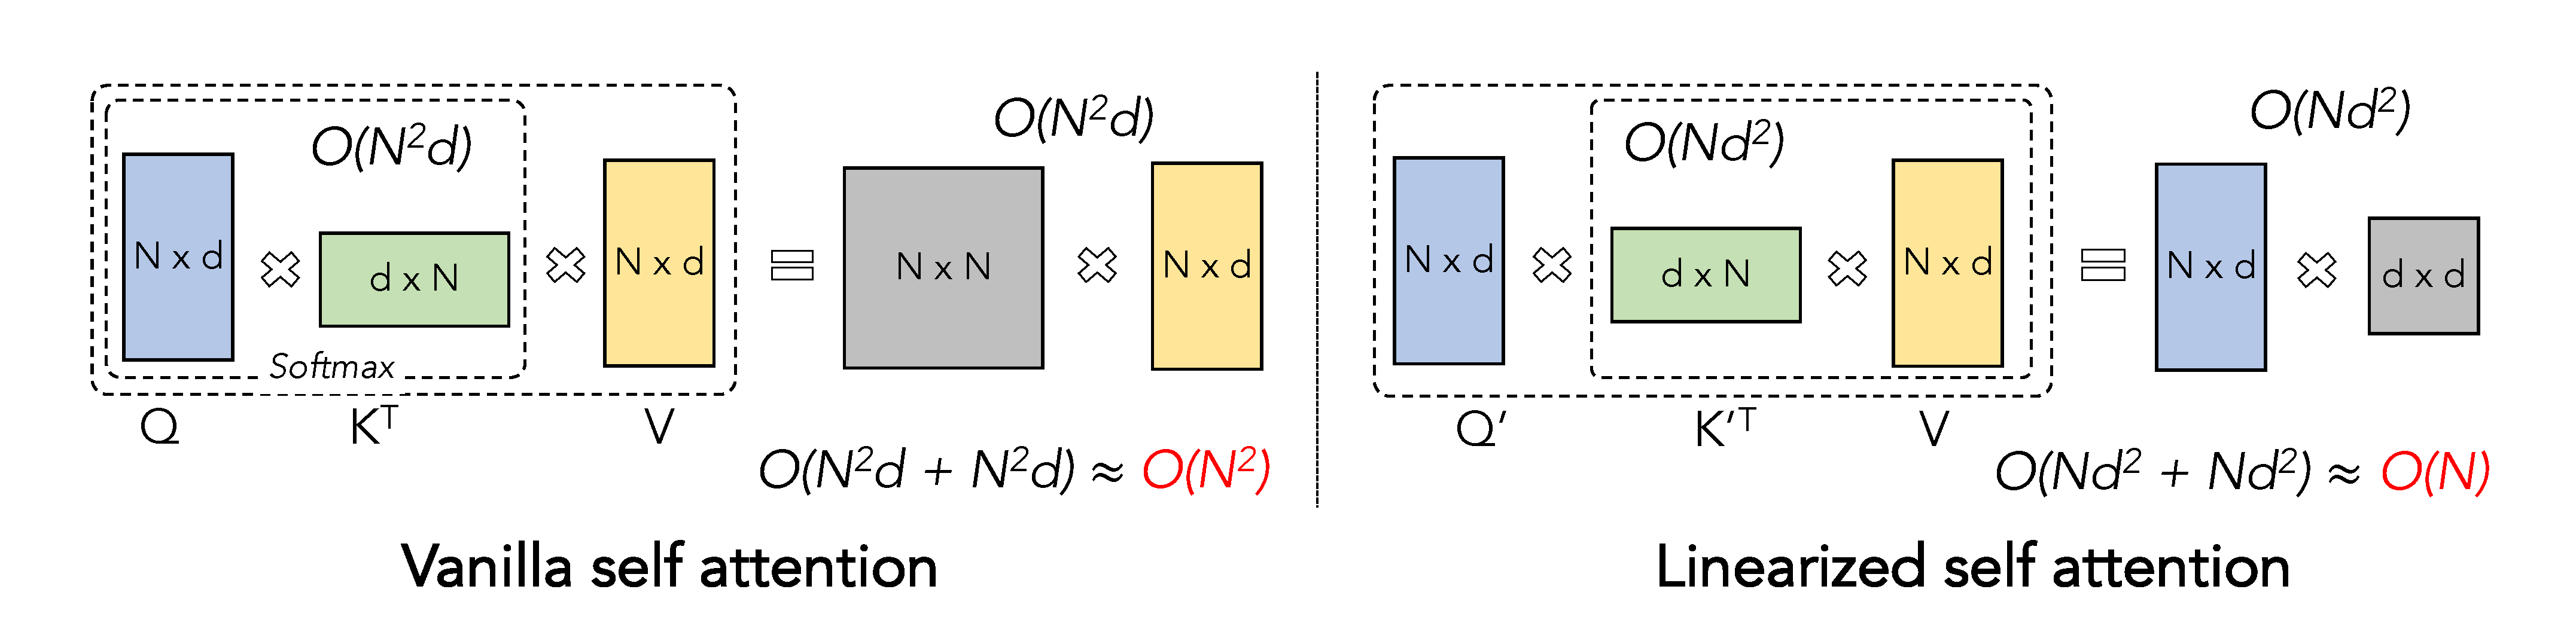
\includegraphics[width=1\linewidth]{figs/cosformer/linear3.pdf}}
\vspace{-10mm}
\end{center}
\caption{基于原始自注意力机制的计算过程(左)和线性化注意力机制的计算过程(右)。输入长度为 $N$,特征维度为 $d$,其中 $d\ll N$。同一框中的张量相关联用于计算。线性化的公式实现了 $O(N)$ 的时间和空间复杂度。摘自~\cite{zhen2022cosformer}}
\vspace{-4mm}
\label{fig: linear}
\end{figure}
\vspace{-2mm}


\subs{指数移动平均(EMA)}
\label{subsec:ema}
移动平均是一种经典的序列数据建模方法,在时间序列数据中广泛用于平滑短期波动并突出长期趋势或周期。指数移动平均(EMA)是移动平均的一种特殊情况,它应用了指数衰减的加权因子。
沿用 ~\ref{subsec:attention} 中对输入输出序列的符号,EMA 可以递归地表示为 $\boldsymbol{Y}$:
\begin{equation}
\label{eq:ema}
\mathbf{y}_t = \boldsymbol{\alpha} \odot \mathbf{x}_t + (1 - \boldsymbol{\alpha}) \odot \mathbf{y}_{t-1},
\end{equation}
其中 $\boldsymbol{\alpha} \in (0, 1)^{d}$ 是 EMA 系数,表示权重减小的程度,$\odot$ 是逐元素乘积。
较高的 $\boldsymbol{\alpha}$ 会更快地衰减旧观测值的权重。EMA偏好于局部依赖关系,并限制了远距离依赖关系。尽管在 \eqref{eq:ema} 中采用了循环形式,EMA 的计算事实上可以表示为 $n$ 个独立的卷积操作,可以使用快速傅里叶变换(FFT)高效计算~\cite{ma2023mega}。

在 \ref{subsec:mega} 中,我们将介绍一种将 EMA 嵌入注意力计算中的计算方式 MEGA,并进一步给出具有线性时间复杂度近似算法 MEGA-chunk(\ref{subsec:mega-chunk})。
\s{现有方法介绍}

在这一节,我们介绍 CosFormer(\ref{subsec:cosformer}),LARA(\ref{subsec:lara}),Skyformer(\ref{subsec:skyformer}) 和 MEGA(\ref{subsec:mega}) 的基本原理。

    \subs{Cosformer}
\label{subsec:cosformer}
\subsubs{Softmax的两个关键属性}
CosFormer\cite{zhen2022cosformer}经验性地确定了softmax操作的两个关键属性,这些属性对其性能可能起到重要作用:
1)它确保注意力矩阵$A$中的所有值都是非负的;
2)它提供了一个非线性重新加权机制,用于集中注意力连接的分布并稳定训练\cite{titsias2016one}。

基于上述性质,Cosformer完全放弃了 softmax 归一化,同时仍然具有非负性和重新加权机制。它包含两个主要组件:线性投影内核 $\phi_{linear}$ 和基于 cos 的重新加权机制。

\subsubs{线性投影内核$\phi_{\text{linear}}$}
回顾注意力的一般形式
\begin{equation}
   \mathcal{O} = \mathcal{A}(x) = \left[\mathcal{O}_1,\hdots, \mathcal{O}_N \right]^T, \quad \mathcal{O}_i
 = \sum_j \frac{\mathcal{S}(Q_i,K_j)}{\sum_j \mathcal{S}(Q_i,K_j)}V_j,
\end{equation}
定义线性相似度为:
\begin{equation}
\mathcal{S}(Q,K)=\mathrm{s}(\phi_{\text{linear}}(Q),\phi_{\text{linear}}(K))=\mathrm{s}(Q',K')
\label{eq:qk}
\end{equation}
其中$\phi_{\text{linear}}$是将查询$Q$和键$K$映射到我们所需表示$Q'$和$K'$的转换函数,
$\mathrm{s}$是一个可以线性分解的函数,用于衡量$Q'$和$K'$之间的相似性。
具体而言,为了确保完全正的注意力矩阵$A$并避免聚集负相关信息,我们采用$\mathrm{ReLU}(\cdot)$作为转换函数,从而有效消除负值:
\begin{equation}
\textstyle{
\phi_{\text{linear}}(x) = \mathrm{ReLU}(x)
}
\end{equation}
由于$Q'$和$K'$只包含非负值,可以直接计算它们的点积$s(x,y) =xy^T, x,y\in \mathbb R^{1\times d}$,然后进行逐行归一化以计算注意力矩阵:
\begin{equation}
\textstyle{
\mathcal{O}i = \frac{\sum^{N}{j=1}f(\phi_{\text{linear}} (Q_i), \phi_{\text{linear}}({K_j})) V_j}{\sum^{N}{j=1}f(\phi{\text{linear}} (Q_i), \phi_{\text{linear}}({K_j}))} = \frac{\sum^{N}{j=1}(\mathrm{ReLU} (Q_i) \mathrm{ReLU}({K_j})^T) V_j}{\sum^{N}{j=1}(\mathrm{ReLU} (Q_i) \mathrm{ReLU}({K_j})^T)}
}
\end{equation}

基于公式
\begin{equation}
\textstyle{
    O_i = \frac{\sum^{N}_{j=1}(\phi (Q_i) \phi({K_j})^T) V_j}{\sum^{N}_{j=1}(\phi (Q_i) \phi({K_j})^T)}.
\label{eq: rewrite att},
}\end{equation}
重新排列点积的顺序,得到以线性复杂度表示的提出的注意力公式:
\begin{equation}
\textstyle{
\label{eq: relu attention}
\mathcal{O}i = \frac{\mathrm{ReLU} (Q_i) \sum^{N}{j=1}\mathrm{ReLU}({K_j})^T V_j}{\mathrm{ReLU} (Q_i)\sum^{N}_{j=1} \mathrm{ReLU}({K_j})^T}
}
\end{equation}

\vspace{-2mm}

\subsubs{基于余弦的重加权机制}
\cite{titsias2016one, gao2017properties} 指出,通过 softmax attention 引入的非线性重新加权机制,可以集中注意力权重的分布,从而稳定训练过程。\cite{zhen2022cosformer}还通过实验证明,这种机制可以惩罚远距离连接并在某些情况下强制局部性。事实上,这种局部性偏差,即大部分上下文依赖关系来自相邻的标记,在下游自然语言处理任务中普遍观察到~\cite{clark2019does, kovaleva2019revealing},如图~\ref{fig: reweight}~(1)所示。

基于上述假设,还需要实现 softmax 的第二个性质,即一种可分解的重新加权机制,能够向注意力矩阵引入最近性偏差。因此,Cosformer提出了一种基于余弦的重新加权机制,因为它完全符合上述目的:1)Ptolemy 定理确保了余弦权重可以分解为两个求和项;2)如图~\ref{fig: reweight}(4)所示,余弦函数在相邻的标记上放置更多的权重,从而强制实现局部性。另外,通过比较图\ref{fig: reweight}~(2)和(3)中的注意力矩阵,可以发现相较于没有重新加权机制的情况,Cosformer更加强调局部性。

\begin{figure}[t]
   \begin{center}
   {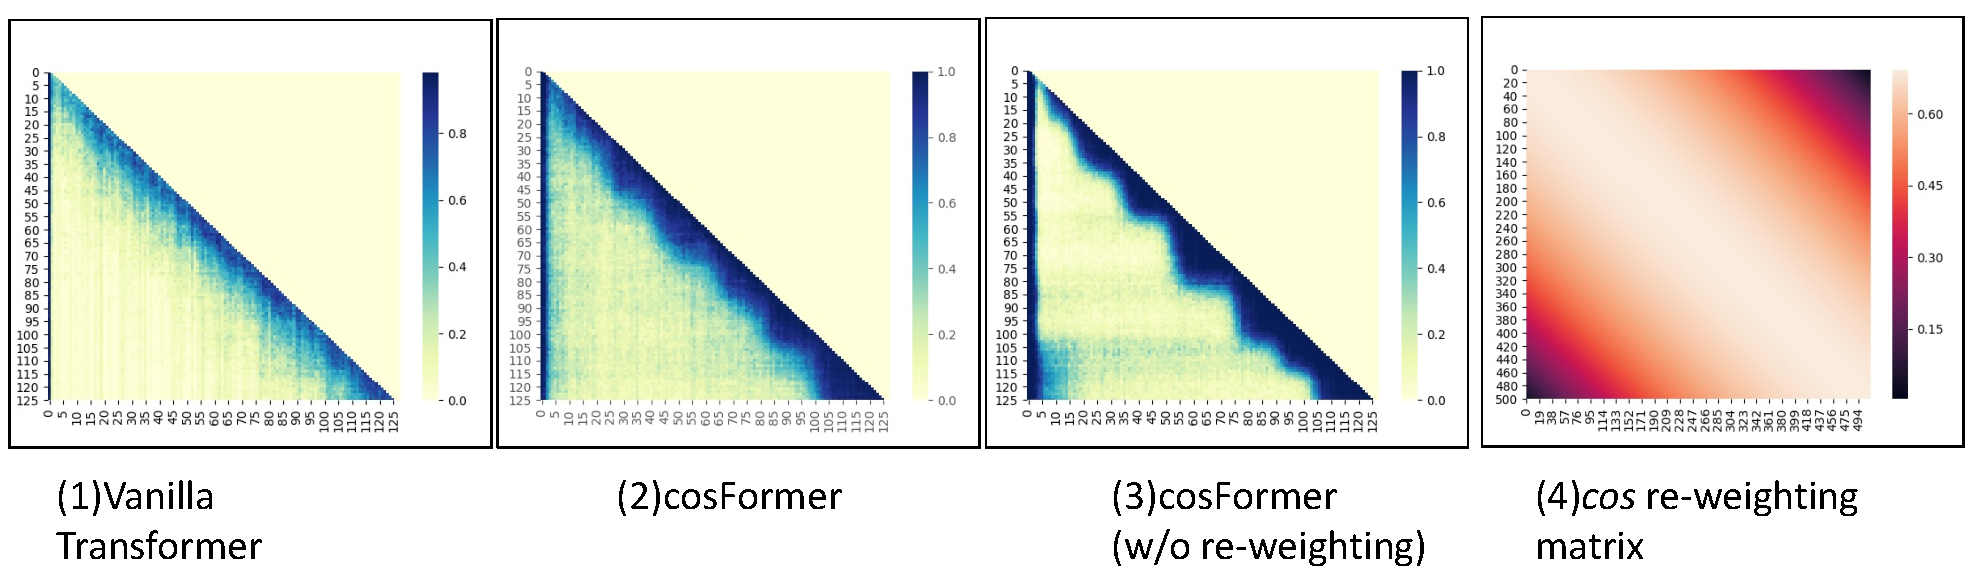
\includegraphics[width=1\linewidth]{figs/cosformer/reweight.pdf}} 
   \vspace{-8mm}
   \end{center}
\caption{(1): Vanilla Transformer的注意力矩阵。(2): Cosformer 的注意力矩阵。(3): 没有重新加权机制的 Cosformer 的注意力矩阵。(4): 基于余弦距离的矩阵可视化。在重新加权后,我们可以看到注意力矩阵的对角区域具有更平滑的注意力分布,呈现出类似于Vanilla Transformer的模式,有助于稳定训练。摘自~\cite{zhen2022cosformer}}
\vspace{-2mm}
   \label{fig: reweight}
\end{figure}

具体而言,结合~\eqref{eq:qk},带有余弦重新加权的模型定义为:
\begin{equation}
\textstyle{
s(Q_i^{'}, K_j^{'})
= Q_{i}^{'}K_{j}^{'T}\cos\left(\frac{\pi}{2} \times \frac{i-j}{M} \right)
}
\end{equation}
\cite{zhen2022cosformer}利用 Ptolemy 定理将这个公式分解为:
\scriptsize
\begin{equation}
\begin{aligned}
Q_{i}^{'}K_{j}^{'T}\cos\left(\frac{\pi}{2} \times \frac{i-j}{M} \right) 
&=Q_{i}^{'}K_{j}^{'T}\left(\cos\left(\frac{\pi i}{2M}\right)\cos\left(\frac{\pi j}{2M}\right) + \sin\left(\frac{\pi i}{2M}\right)\sin\left(\frac{\pi j}{2M}\right)\right)\ \\
&= \left(Q_{i}^{'} \cos \left(\frac{\pi i}{2M}\right)\right)\left(K_{j}^{'}\cos\left(\frac{\pi j}{2M}\right)\right)^{T} + \left(Q_{i}^{'}\sin\left(\frac{\pi i}{2M}\right)\right)\left(K_{j}^{'} \sin\left(\frac{\pi j}{2M}\right)\right)^{T}
\end{aligned}
\end{equation}
\normalsize

其中,$\small{i ,j= 1,...,N, M \geq N}$,$\small{Q^{'} = \mathrm{ReLU}(Q),K^{'} = \mathrm{ReLU}(K)}$。
令 $\small{Q_{i}^{\cos} =Q_{i}^{'} \cos \left(\frac{\pi i}{2M}\right)}$,$\small{Q_{i}^{\sin} =Q_{i}^{'} \sin \left(\frac{\pi i}{2M}\right)}$,

$\small{K_j^{\cos} =K_{j}^{'}\cos\left(\frac{\pi j}{2M}\right)}$,$\small{K_j^{\sin} =K_{j}^{'}\sin\left(\frac{\pi j}{2M}\right)}$,
则提出的注意力模块的输出可以表示为:
\begin{equation}
\label{eq appendix}
\textstyle{
O_i = \frac{\sum_{j=1}^N f(Q_i^{'}, K_j^{'}) V_j}{\sum^{N}{j=1} f(Q_i^{'}, K_j^{'}) }
= \frac{\sum{j=1}^N Q_{i}^{\cos} \left( \left( K_j^{\cos} \right)^TV_j \right)+\sum_{j=1}^N Q_{i}^{\sin} \left(\left( K_j^{\sin} \right)^T V_j \right)}{\sum_{j=1}^N Q_{i}^{\cos} \left( K_j^{\cos} \right)^T+\sum_{j=1}^N Q_{i}^{\sin} \left( K_j^{\sin} \right)^T },
}
\end{equation}

其中 $O_i$ 是注意力模块输出的序列中第 $i$ 个位置的值。
不失一般性,Cosformer的时间复杂度是线性的,表示为:
\begin{equation}
\textstyle{
\mathcal{O} = \mathcal{S}(Q, K)V
=(Q^{\cos}K^{\cos} + Q^{\sin}K^{\sin})V
=Q^{\cos}(K^{\cos}V) + Q^{\sin}(K^{\sin}V)
}
\end{equation}

从位置编码的角度来看, Cosformer 可以看作是一种将相对位置偏差引入高效Transformer的新方法。
    \subs{LARA(线性随机注意力)}
\label{subsec:lara}

本节我们介绍了一种改进的 softmax 注意力估计器—LARA。受随机特征注意力(RFA)\cite{peng2021random,}和随机注意力(RA)\cite{choromanski2020rethinking} 之间的差异的启发,LARA 通过采用多个提议来推广 RFA 的重要性采样公式。这种策略不仅可以以更细粒度的方式捕捉查询信息,还允许模型以特定于查询的方式估计 softmax 注意力。并且Lara可以实现计算重用,借助自标准化重要性采样可以实现线性复杂度计算。

\subsubs{多提议重要性采样}
\label{ssec:lara_mis}
RA和RFA都旨在估计期望 $\mathbb{E}_{p_n(\omega)}\left[f_n(\omega)\right]
 =  \mathbb{E}_{p_n(\omega)}\!\!\left[\frac{\xi(q_n,\omega)^\top \!\sum_{m=1}^M\xi(k_m, \omega) v_{m}^{\top}}{ \xi(q_n,\omega)^\top \!\sum_{m'=1}^M\xi(k_{m'}, \omega)}\right]\!
 = \mathsf{SoftmaxAttn}(q_n, K,V)$
它们之间的主要区别在于RA为每个查询从不同的分布中采样,而RFA对所有查询使用相同的提议分布。为了兼顾两者的优势,LARA采用一组$C$($C \ll N$)提议分布$\{{q_c(\omega)}\}_{c=1}^C$进行估计,其中每个提议分布依赖于一部分查询。

这种策略不仅能够以更细粒度的方式处理查询信息,还允许模型以查询特定的方式估计softmax注意力,这是RA的关键优势。具体而言,由于每个查询都有几个提议可用,并且这些提议可能相互提供互补的信息,可以通过多重重要性采样\cite{veach1995optimally}将它们组合起来。对于每个查询,MIS估计的形式如下(注意:这里假设每个提议分布只抽取一个样本。更一般的处理方式允许从每个提议分布抽取任意数量的样本):
\begin{equation}
\mathbb{E}_{p_n(\omega)}\left[f_n(\omega)\right] \approx \sum_{c=1}^C \alpha_{nc}(\omega_c) \frac{p_n(\omega_c)}{q_c(\omega_c)}f_n(\omega_c)\label{eqn:lara:mis}
\end{equation}
其中 $\omega_c \sim q_c(\omega)$,$c=1,\dots,C$,$\{{\alpha_{nc}(\cdot)}\}_{c=1}^C$ 是\emph{加权函数}。如果对于任意 $\omega$ 都有 $\sum_{c=1}^C \alpha_{nc}(\omega) = 1$,那么由\cite{veach1995optimally}可知,MIS估计是无偏的。
% \footnote{严格来说,为了使MIS估计无偏,还需要加权函数对于任何使 $p_n(\omega) = 0$ 的 $\omega$ 都为零,尽管在LARA的设置中这是显然成立的。}
直观地说,MIS首先使用每个提议的单独重要性采样估计值,然后根据\emph{查询特定}的加权函数对它们进行平均。

理想情况下,第 $n$ 个加权函数集合 $\{{\alpha_{nc}(\cdot)}\}_{c=1}^C$ 应专门用于处理第 $n$ 个查询。为实现这一目标,加权函数应对应于相应查询的最优函数(即最小化估计方差)。最优加权函数的形式如下:
\begin{equation}
\alpha^*_{nc}(\omega_c) =
\frac{q_c(\omega_c)}{\sum_{c'=1}^C q_{c'}(\omega_c)} + q_c(\omega_c)\left(r_{nc}(\omega_c) - \sum_{c=1}^C\frac{q_c(\omega_c)}{\sum_{c'=1}^C q_{c'}(\omega_c)}r_{nc}(\omega_c)\right).
\end{equation}
这里 $r_{nc}(\cdot)$ 大致与 $q_c(\cdot)$ 与查询特定最优提议之间的接近程度成正比。直观地说,最优加权函数由两项组成。第一项与查询无关,第二项是查询特定的校正项。校正项由 $r_{nc}(\cdot)$ 与其由 $q_c(\cdot)$ 加权的平均值之间的差异定义;因此,如果 $r_{nc}(\cdot)$ 较大,则校正项将为正,推动第 $c$ 个提议的权重更高,反之亦然。

在大多数情况下,应用最优加权函数是不可行的,因为 $r_{nc}(\cdot)$ 的闭式形式是不可用的。因此,LARA通过以下形式来近似最优加权函数:
\begin{equation}
\alpha_{nc}(\omega_c) = \frac{q_c(\omega_c)}{\sum_{c'=1}^C q_{c'}(\omega_c)} + r'_{nc} - \frac{1}{C}\sum_{c=1}^Cr'_{nc},\label{eqn:lara:opt_weighting_function}
\end{equation}
其中 $r'_{nc}$ 衡量了提议 $q_c$ 对第 $n$ 个查询的偏好程度。为了可行性,LARA将 $r'_{nc}$ 实现为第 $n$ 个查询与第 $c$ 个查询子集的表示之间的归一化相似性。还将提议密度 $q_c(\omega)$ 和 $r'_{nc}$ 的计算分离,以使与查询无关和查询特定项的贡献可以相互独立。请注意,由于 $\sum_{c=1}^C \alpha_{nc}(\omega) = 1$,Eq.\ref{eqn:lara:opt_weighting_function}仍然确保了MIS估计的无偏性(或一致性)。

\subsubs{实现线性时间和空间复杂度}
\label{ssec:lara_snis}
根据MIS估计器(\ref{eqn:lara:mis}),在每个提议下的键-值统计信息可以预先计算一次,然后在所有查询中重复使用。这意味着RFA中的计算重用是可行的,从而实现了线性复杂度。

现在唯一剩下的问题是MIS估计器仍然需要对每个查询明确评估密度 
$p_n(\omega)=\sum_{m=1}^M \pi_{m} \mathcal{N}(\omega; q_n + k_m, \mathbf{I})$,
这会导致二次复杂度。这是因为 $p_n(\omega)$ 是一个具有 $M$ 个分量的高斯混合,总共需要 $O(NM)$ 次计算。LARA展示了一种自标准化版本的MIS,可以将复杂度进一步降低到线性。混合密度 $p_n(\omega)$ 可以等价地表示为
\begin{equation}
\textstyle{
p_n(\omega) = \frac{\mathcal{N}(\omega;0,\mathbf{I}) \xi(q_n,\omega)^\top \sum_{m=1}^M \xi(k_{m}, \omega)}{\sum_{m'=1}^M \exp\left(q_n^\top k_{m'}\right)} = \frac{\tilde{p}n(\omega)}{Z_p}
}
\end{equation}
我们的关键观察是,现在分子包含了一个线性化的随机映射点积,可以预先计算并在所有查询中重复使用,而分母类似于常规softmax注意力中的归一化常数,并且只能在二次时间内计算。幸运的是,如果采用\emph{自标准化}估计器,
\begin{equation}
\label{eqn:lara}
\textstyle{
\mathbb{E}{p_n(\omega)}\left[f_n(\omega)\right] \approx
\frac{\sum_{c=1}^C\alpha_{nc}(\omega_c)\frac{\tilde{p}n(\omega_c)}{q_c(\omega_c)} f_n(\omega_c)}{\sum{c=1}^C\alpha_{nc}(\omega_c)\frac{\tilde{p}n(\omega_c)}{q_c(\omega_c)}} \
= \mathsf{LARA}\left(q_{n},K,V\right)
}
\end{equation}
所得到的估计器是一致的,并且具有与RFA类似的线性复杂度。
    \subs{Skyformer}
这一节我们介绍 Skyformer 近似计算加速的原理。
\label{subsec:skyformer}
\subsubs{核化注意力}
\label{sec:kernel_attn}
Softmax注意力的一个显著优点是允许元素仅和序列中的少量重要元素发送关联,
高斯核函数可以起到类似的作用。高斯核函数的表达式为$\kappa(Q_i,  K_j) := \exp \left(-\|Q_i - K_j\|^2 / 2 \right)$。
通过这个表达式,对于查询中的元素$i$,当$K_j$接近于$Q_i$时,高斯核赋予元素$j$较大的注意力。
基于距离的加权分配正是核方法强大的一个重要原因。
核化注意力的形式也导致了自动归一化。

核化注意力使用高斯核函数 $\kappa$ 替代了普通自注意力中的softmax结构,新的注意力模型定义如下:
\begin{equation}
\text{Kernelized-Attention}(Q,K,V) = C V = \kappa\left(\frac{Q}{p^{1/4}}, \frac{K}{p^{1/4}} \right) V,
\end{equation}
其中$n$乘$n$矩阵$C$定义为核化注意力得分矩阵$\kappa(Q / p^{1/4}, K / p^{1/4})$,而 $V$ 则是一般意义下的值向量。

由此,新的注意力模型可以用未归一化的注意力矩阵$A$表示为
\begin{equation*}
\text{Kernelized-Attention}(Q,K,V) = \left( D_Q^{-1/2} \cdot A \cdot D_K^{-1/2} \right) V,
\end{equation*}
其中$D_Q$(对应$D_K$)是一个对角矩阵,其元素为$(D_Q)_{ii} = \exp\left( \frac{\|Q_i\|^2}{\sqrt{p}} \right)$ ,相应地,$(D_K)_{ii} = \exp \left( \frac{\|K_i\|^2}{\sqrt{p}} \right)$),$\forall i \in \mathbb{N}$。
Skyformer指出,核化注意力模型可以看作原始自注意力的一种变体,它将矩阵$A$归一化为$D^{-1} A$的形式。
这种归一化使得核化注意力具有比自注意力更合理的条件数,从而有助于模型训练的稳定性。

\subsubs{改进的\textit{Nystrom}方法}
\label{sec:nystrom}

Skyformer将\textit{Nystrom}方法应用于非对称的经验核矩阵$B$。该核矩阵是由任意半正定核$\phi(\cdot, \cdot)$构造而成的。

具体而言,给定两个不同的$n$行$p$列设计矩阵$Q$和$K$,$B$中第$i$行第$j$列的元素$b_{ij}$等于$\phi(Q_i, K_j)$,其中$Q_i$是$Q$的第$i$行,$K_j$是$K$的第$j$行。
如果取用 $\phi$ 为高斯核,我们就可以得到对上述高斯核矩阵$C = \kappa(Q / p^{1/4}, K / p^{1/4})$的近似,从而完成对核化注意力$C V$输出的低秩近似。

接下来的问题就是如何去计算经验核矩阵 $B$。由于$B$不是半正定矩阵,第一步是将该矩阵补充成一个半正定矩阵$\bar{B}$
\begin{equation}
\label{eqn:concat}
\bar{B} = \phi \left(
\begin{pmatrix}
Q \
K
\end{pmatrix},
\begin{pmatrix}
Q \
K
\end{pmatrix} \right).
\end{equation}
然后,通过Nystorm方法,用$\tilde{\bar{B}}$近似$\bar{B}$:
\begin{align}
\label{eqn:tilde_bar}
\tilde{\bar{B}} = \bar{B} S (S^{T} \bar{B}\textbf{S})^{\dagger} \textbf{S}^{T}\bar{B},
\end{align}
其中$S$是一个由均匀子采样矩阵构成的$2n$行$d$列矩阵,$(\cdot)^\dagger$ 表示Moore-Penrose广义逆。

最终,Skyformer 对 $B$ 的近似结果为
\begin{align}
\label{eqn:approx}
\tilde{B} = (I, 0) \tilde{\bar{B}} (0, I)^T.
\end{align}
Skyformer 指出,由于下述不等式成立,
\begin{align*}
|B - \tilde{B}| = |(I, 0) (\bar{B} - \tilde{\bar{B}}) (0, I)^T| \leq |\bar{B} - \tilde{\bar{B}}|,
\end{align*}
原始矩阵$B$可以很好地被$\tilde{B}$近似,从而将近似非半正定矩阵$B$的任务归结为对半正定矩阵$\bar{B}$进行良好的近似。
Skyformer 指出,从经验来看,核矩阵$\bar{B}$中的特征值通常快速衰减,从而在长尾部分存在许多较小的特征值。此时,低秩矩阵在谱范数意义下可以很好地近似原始矩阵,如 $\bar{B}$的截断奇异值分解可以很好地近似$\bar{B}$。
    \subs{MEGA(门控移动平均注意力)}
\label{subsec:mega}

在本节中,我们介绍 ~\cite{ma2023mega} 提出的门控移动平均注意力(Moving Average Equipped Gated Attention,MEGA)方法。
我们将首先介绍多维阻尼指数移动平均(Multi-dimensional Damped EMA)(\ref{subsubsec:mddema}),和门控注意力层(\ref{subsubsec:mega})。接下来,我们引入 MEGA-chunk 将输入序列进行固定大小的分块,从而将序列处理的复杂性从平方降低到线性(\ref{subsec:mega-chunk})。

\subsubs{多维阻尼指数移动平均}
\label{subsubsec:mddema}

MEGA 引入了一种改进的标准指数移动平均(EMA)方法,称为多维阻尼指数移动平均。~\cite{svetunkov2016complex}指出,通过减小先前元素和当前元素间的关联权重($\boldsymbol{\alpha}$ 和 \eqref{eq:ema} 中的 $1 - \boldsymbol{\alpha}$),可以实现稳健的依赖建模。受此启发,MEGA 在经典的EMA中引入阻尼因子,从而允许模型减小先前时间步元素的权重:
\begin{equation}
\label{eq:damping}
\mathbf{y}_t = \boldsymbol{\alpha} \odot \mathbf{x}_t + (1 - \boldsymbol{\alpha} \odot \boldsymbol{\delta}) \odot \mathbf{y}_{t-1},
\end{equation}
其中 $\boldsymbol{\delta} \in (0, 1)^{d}$ 是阻尼因子。

为了进一步增强 EMA 的表示能力,MEGA 设计了多维阻尼移动平均机制。首先,通过扩展矩阵 $\boldsymbol{\beta} \in \mathbb{R}^{d\times h}$ 将输入序列 $\boldsymbol{X}$ 的每个维度的标量单独扩展到 $h$ 维。对于每个维度的标量 $j \in \{1, 2, \ldots, d\}$:
\begin{equation}
\mathbf{u}^{(j)}_t = \boldsymbol{\beta}_j \mathbf{x}_{t,j}
\end{equation}
其中 $\boldsymbol{\beta}_j \in \mathbb{R}^{h}$ 是 $\boldsymbol{\beta}$ 的第 $j$ 行,  $\mathbf{u}^{(j)}_t \in \mathbb{R}^{h}$ 是第 $j$ 维在时间步 $t$ 展成的 $h$ 维向量.

相应地,我们将$\boldsymbol{\alpha}$和$\boldsymbol{\delta}$的形状从一维向量扩展为二维矩阵,即$\boldsymbol{\alpha}$,$\boldsymbol{\delta} \in \mathbb{R}^{d\times h}$,其中$\boldsymbol{\alpha}_j$,$\boldsymbol{\delta}_j \in \mathbb{R}^{h}$ 分别表示$\boldsymbol{\alpha}$和$\boldsymbol{\delta}$的第$j$行。
然后,对于每个维度$j$,在$h$维隐空间上应用阻尼EMA:
\begin{align}
\label{eq:mddema}
\mathbf{h}^{(j)}_t & = \boldsymbol{\alpha}_j \odot \mathbf{u}^{(j)}_t + (1 - \boldsymbol{\alpha}_j \odot \boldsymbol{\delta}_j) \odot \mathbf{h}^{(j)}_{t-1} \nonumber \\
\mathbf{y}_{t,j} & = \boldsymbol{\eta}^T_j \mathbf{h}^{(j)}_t
\end{align}
其中$\mathbf{h}^{(j)}_t \in \mathbb{R}^{h}$ 是时间步$t$时第$j$维度的EMA隐藏状态。
$\boldsymbol{\eta} \in \mathbb{R}^{d\times h}$ 是投影矩阵,将$h$维隐藏状态映射回$1$维输出$\mathbf{y}_{t,j} \in \mathbb{R}$。$\boldsymbol{\eta}_j \in \mathbb{R}^{h}$ 是$\boldsymbol{\eta}$的第$j$行。
从\eqref{eq:mddema}中得到的输出$\boldsymbol{Y}$被表示为$\boldsymbol{Y} \stackrel{\Delta}{=} \mathrm{EMA}(\boldsymbol{X})$。
由于不需要显式计算 $\mathbf{h}^{(j)}_t$ 来获取输出 $\mathbf{y}_{t,j}$,时间和空间复杂度与标准EMA相似。

\begin{figure}[!t]
\centering
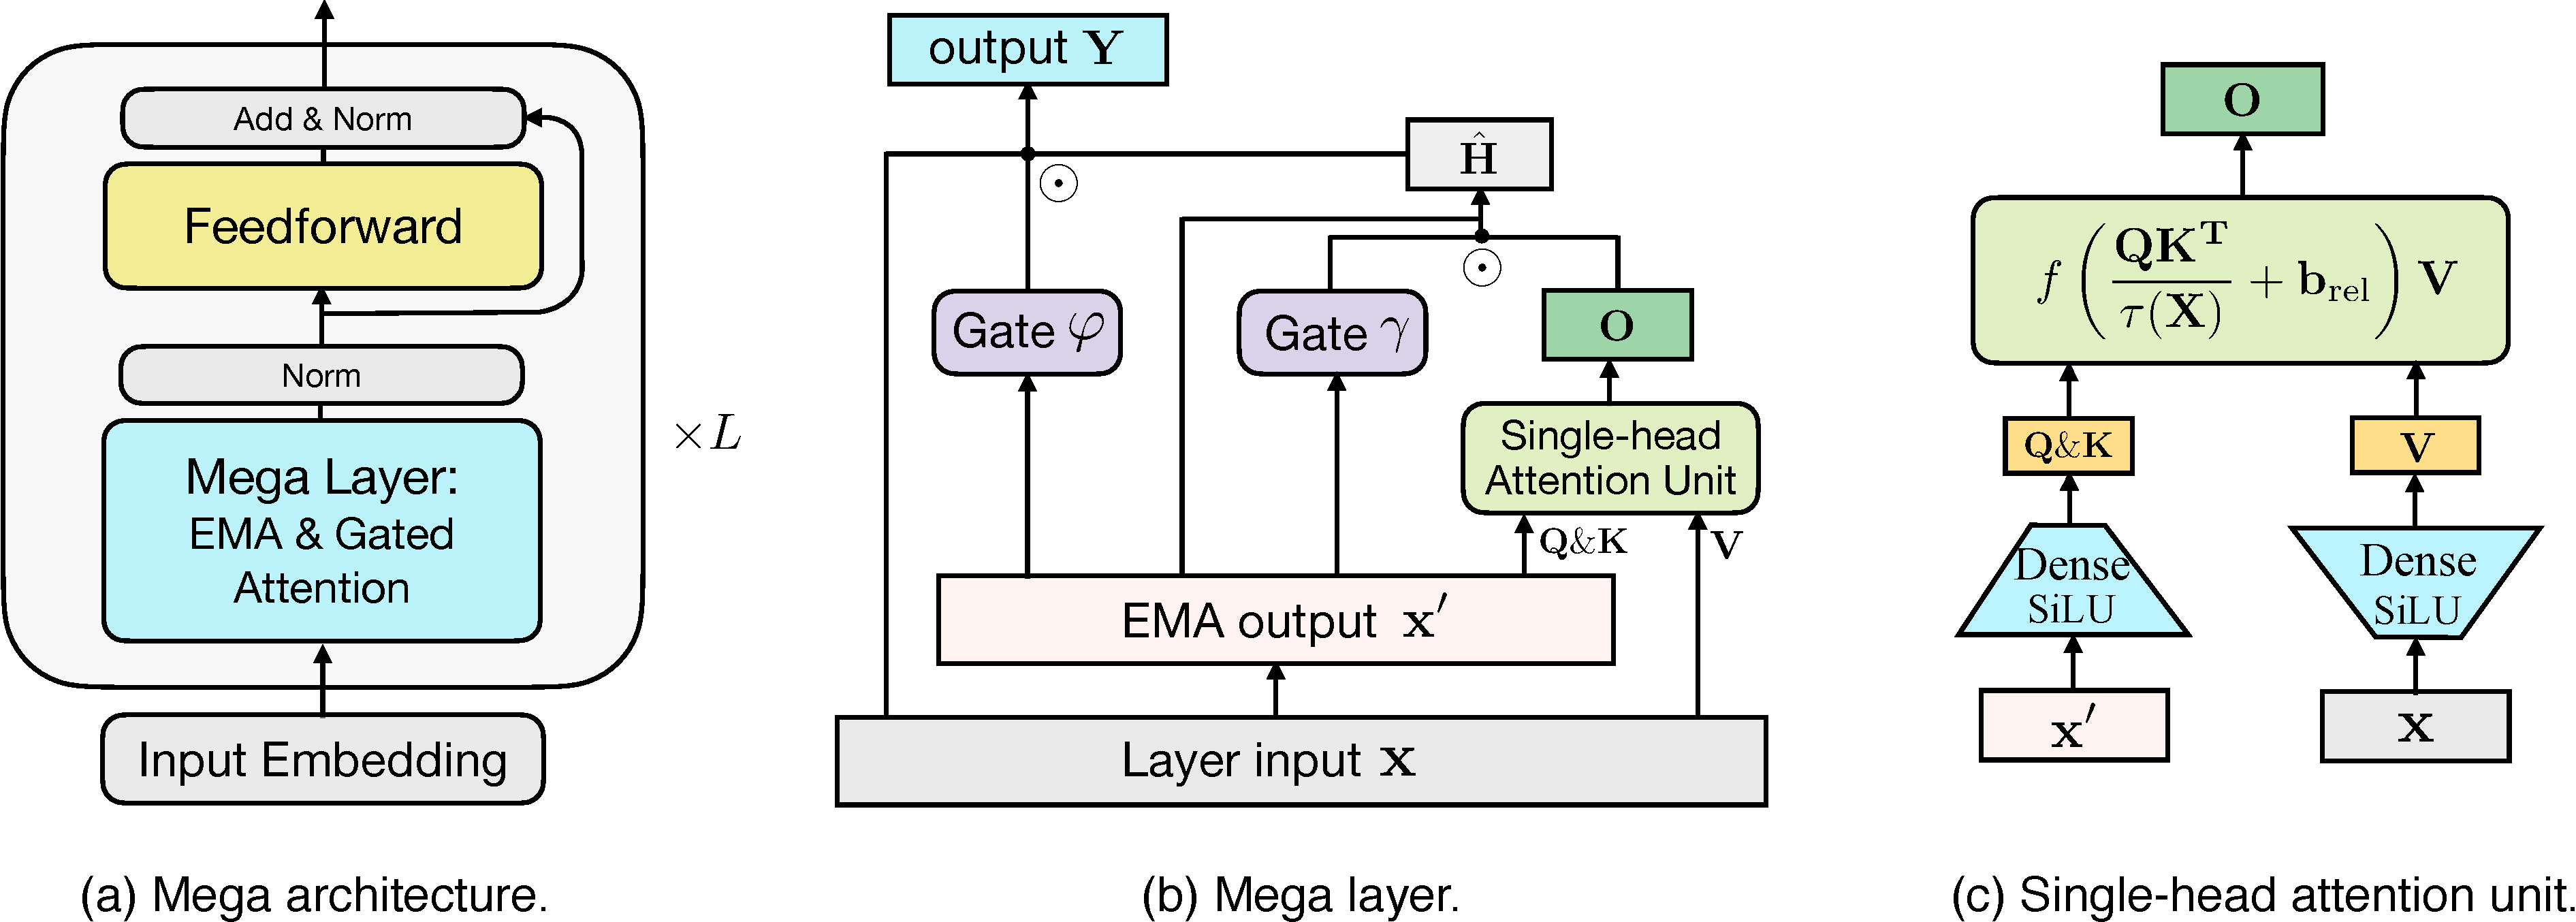
\includegraphics[width=0.99\textwidth]{figs/mega/model.pdf}
\caption{MEGA模型架构。(a) MEGA块。(b) MEGA的门控注意力层。(c) MEGA的单头注意力单元。摘自~\cite{ma2023mega}}
\label{fig:arch}
\end{figure}

\subsubs{MEGA门控注意力层}
\label{subsubsec:mega}
MEGA中的门控注意力机制采用门控循环单元(GRU\cite{cho2014properties})和门控注意力单元(GAU\cite{hua2022transformer})作为骨干结构。具体来说,首先使用\eqref{eq:mddema}中的输出计算GAU中的共享表征:
\begin{align}
\boldsymbol{X}' & = \mathrm{EMA}(\boldsymbol{X}) \qquad & \qquad \in \mathbb{R}^{n\times d} \\
\boldsymbol{Z} & = \phi_{\mathrm{silu}}(\boldsymbol{X}' W_z + b_z) \qquad & \qquad \in \mathbb{R}^{n\times z} \label{eq:z}
\end{align}
其中 $\boldsymbol{X}'$可以被视为编码了上下文信息的表征向量。而
$\boldsymbol{Z}$则是一个$z$维的高效表征。$W_z \in \mathbb{R}^{d\times z}$ 和 $b_z \in \mathbb{R}^{z}$分别是投影矩阵和偏移。
$\phi_{\mathrm{silu}}$是SiLU激活函数~\cite{ramachandran2017swish}。


在GAU之后,通过对$\boldsymbol{Z}$应用每个维度的标量和偏移量来计算查询$\boldsymbol{Q}$和键$\boldsymbol{K}$,而值序列 $\boldsymbol{V}$ 则由原始的$\boldsymbol{X}$直接得到:
\begin{align}
\boldsymbol{Q} & = \boldsymbol{\kappa}_q \odot \boldsymbol{Z} + \boldsymbol{\mu}_q \qquad & \qquad \in \mathbb{R}^{n\times z} \label{eq:query} \\
\boldsymbol{K} & = \boldsymbol{\kappa}_k \odot \boldsymbol{Z} + \boldsymbol{\mu}_k \qquad & \qquad \in \mathbb{R}^{n\times z} \\
\boldsymbol{V} & = \phi_{\mathrm{silu}}(\boldsymbol{X} W_v + b_v) \qquad & \quad \qquad \in \mathbb{R}^{n\times v} \label{eq:value}
\end{align}
这里,$\boldsymbol{\kappa}_q$、$\boldsymbol{\mu}_q$、$\boldsymbol{\kappa}_k$、$\boldsymbol{\mu}_k \in \mathbb{R}^{z}$是可学习的参数。$v$是值序列的输出维度。


注意力的计算如图~\ref{fig:arch}(c)所示,形式化表示为:
\begin{align}\label{eq:attention2}
\boldsymbol{O} & = f \left(\frac{\boldsymbol{Q}{\boldsymbol{K}}^{T}}{\tau(\boldsymbol{X})} + \boldsymbol{b}_{\mathrm{rel}} \right) \boldsymbol{V} \quad & \quad \qquad \in \mathbb{R}^{n\times v}
\end{align}
其中,$\boldsymbol{b}_{\mathrm{rel}} \in \mathbb{R}^{n\times n}$表示相对位置偏置。

类似于 GRU,MEGA引入重置门$\boldsymbol{\gamma}$、更新门$\boldsymbol{\varphi}$,并计算候选激活输出$\boldsymbol{\hat{H}}$。这些概念的含义与GRU中的概念类似。
\begin{align}
\boldsymbol{\gamma} & = \phi_{\mathrm{silu}}(\boldsymbol{X}' W_\gamma + b_\gamma) & \in \mathbb{R}^{n\times v} \label{eq:reset} \\
\boldsymbol{\varphi} & = \phi_{\mathrm{sigmoid}}(\boldsymbol{X}' W_\varphi + b_\varphi) & \in \mathbb{R}^{n\times d} \label{eq:update} \\
\boldsymbol{\hat{H}} & = \phi_{\mathrm{silu}}(\boldsymbol{X}' W_h + (\boldsymbol{\gamma} \odot \boldsymbol{O}) U_{h} + b_h) & \in \mathbb{R}^{n\times d} \label{eq:candidate}
\end{align}
输出$\boldsymbol{Y}$使用更新门$\boldsymbol{\varphi}$计算:
\begin{align}
\boldsymbol{Y} & = \boldsymbol{\varphi} \odot \boldsymbol{\hat{H}} + (1 - \boldsymbol{\varphi}) \odot \boldsymbol{X} \qquad & \qquad \in \mathbb{R}^{n\times d} \label{eq:output}
\end{align}
MEGA子层的图形架构在图~\ref{fig:arch}(b)中可视化。

\subsubs{Laplace注意力函数}
Softmax是注意力函数最常见的选择。而
\cite{so2021searching}提出的平方ReLU函数$f_{\mathrm{relu^2}}(\cdot)$在语言任务上显示出更快的收敛速度和更好的泛化性能~\cite{hua2022transformer}。
然而,$f_{\mathrm{relu^2}}(\cdot)$的一个问题是它的梯度范围没有上界这导致了模型训练不稳定。为了解决这个问题,MEGA提出了一种基于Laplace函数的新注意力函数:
\begin{equation}
\label{eq:laplace}
f_{\mathrm{laplace}}(x; \mu,\sigma) = 0.5 \times \left[1 + \mathrm{erf}(\frac{x - \mu}{\sigma\sqrt{2}}) \right]
\end{equation}
其中 $\mathrm{erf}(x) = \frac{2}{\sqrt{\pi}} \int_0^x e^{-t^2} dt$。MEGA 中,选取$\mu=\sqrt{1/2}$和$\sigma=\sqrt{1/4\pi}$ 从而使得 $f_{\mathrm{laplace}}$ 逼近 $f_{\mathrm{relu}^2}$。


\subsubs{MEGA-chunk}
\label{subsec:mega-chunk}

\begin{figure}[t]
\centering
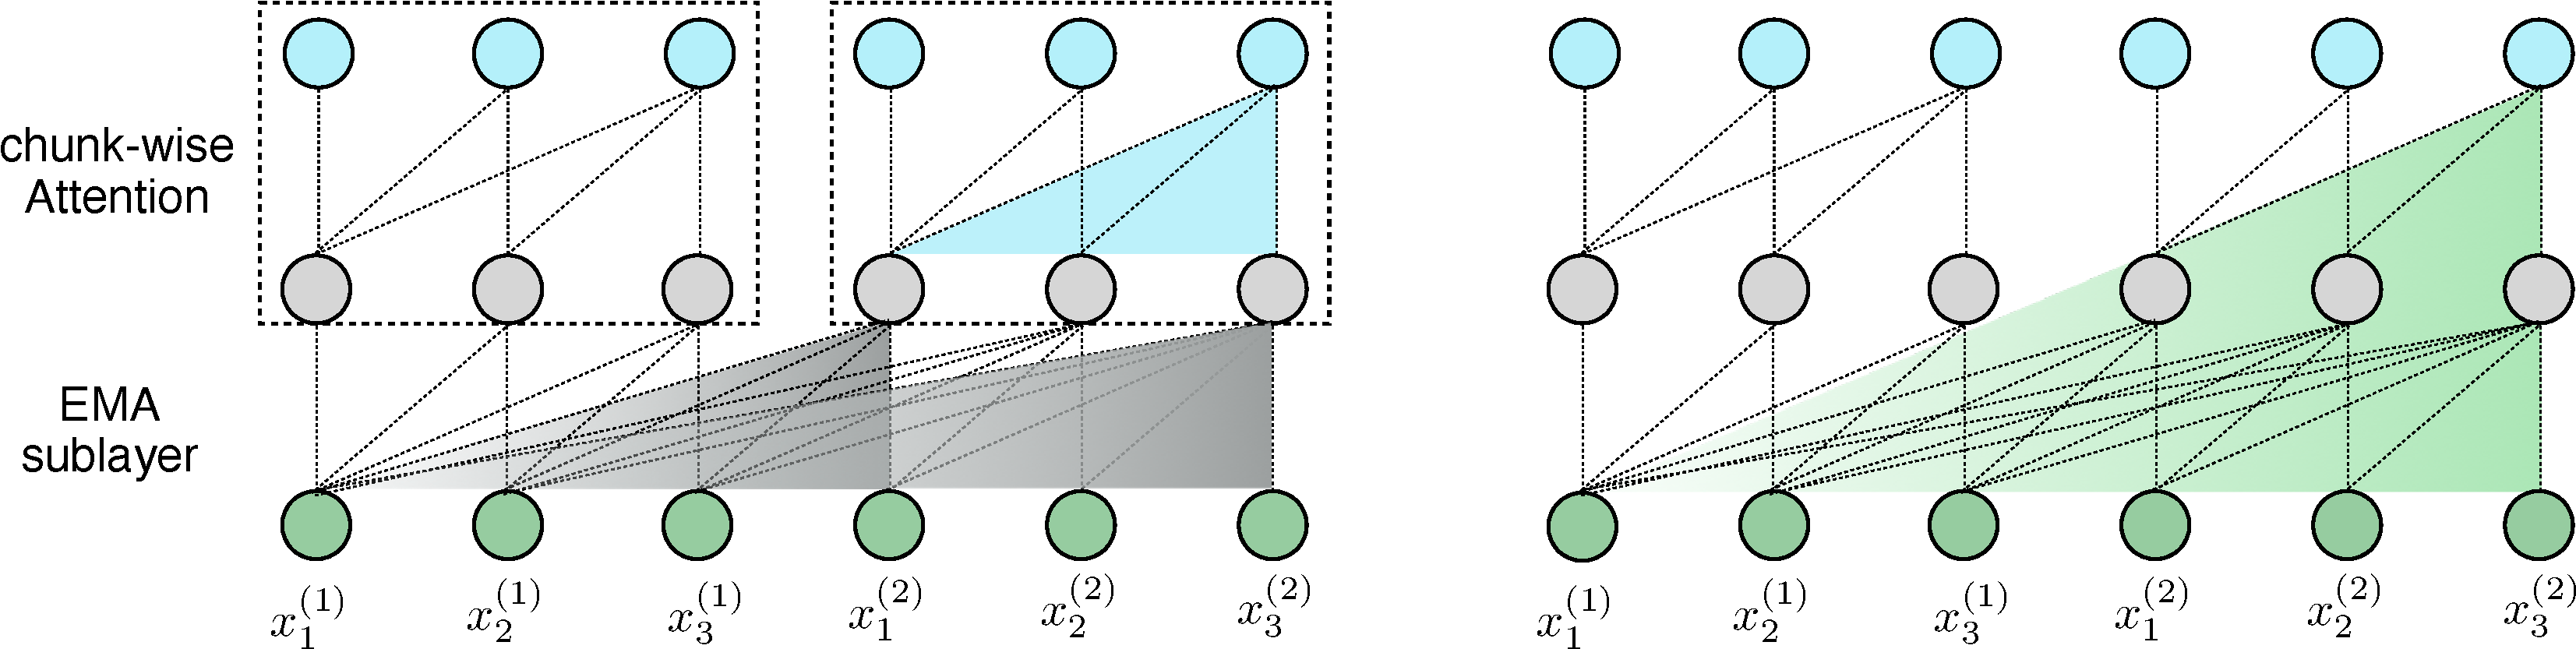
\includegraphics[width=0.99\textwidth]{figs/mega/ema_chunk_attn.pdf}
\caption{$c=3$时,MEGA-chunk 的注意力范围。摘自~\cite{ma2023mega}}
\label{fig:chunk}
\vspace{-3mm}
\end{figure}

进行了以上调整的 MEGA 注意力仍然具有$O(n^2)$ 的时空复杂度,而MEGA方法加速的关键在于将时间复杂度压缩至线性,也就是 MEGA-chunk 方法。具体来说,首先将 (\ref{eq:query}-\ref{eq:value}) 中的$\boldsymbol{Q}$, $\boldsymbol{K}$, $\boldsymbol{V}$ 序列划分为长度为 $c$ 的块,即

\begin{align}
    \boldsymbol{Q} & = \{\boldsymbol{Q}_1, \ldots,  \boldsymbol{Q}_k\} \\
    \boldsymbol{K} & = \{\boldsymbol{K}_1, \ldots,  \boldsymbol{K}_k\} \\
    \boldsymbol{V} & = \{\boldsymbol{V}_1, \ldots,  \boldsymbol{V}_k\} 
\end{align}

其中 $k = \lceil \frac n c \rceil$ 是块的数量。

接下来,每个分块独立进行\eqref{eq:attention2}中的注意力操作。这样整体的注意力复杂度对 $n$ 呈线性,即 $O(kc^2)=O(nc)$。由于在进行分块注意力前,每个时序向量通过 EMA 层捕获了块外的信息,这使其信息收集范围远超一个块的约束范围。如图~\ref{fig:chunk}所示。
    
\s{实验}
    在这一节,我们对上述绍四种 Attention 加速方法的性能进行衡量。我们采用~\cite{tay2021long}中提出的 Long Range Arena 基准比较各方法的建模能力和运行开销。最后,我们也探索了MEGA模型在的部分超参对模型性能的影响。
\subs{实现细节}
\subsubs{数据集}
Long Range Arena 数据集~\cite{tay2021long} 被广泛用于验证模型的长序列建模性能,其从不同角度设计了5种序列建模任务。

文本序列分类任务(Text)。任务采用 IMDB 数据集,输入为字节级表示(而非事先分词)文本,要求模型输出为文本情感的二分类。最大上下文长度为 4K。

结构化操作任务(ListOps)。这一任务测量模型对结构化长序列的建模能力,其输入为一段嵌套的操作序列,要求模型输出操作的结果(输出为0至9,建模为10分类任务),其最长上下文长度为 2K。下面举一个例子对任务进行说明

\begin{verbatim}
    输入 [ MAX 4 3 [ MIN 2 3 ] 1 0 [ MEDIAN 1 5 8 9 2] ]
    输出 5
\end{verbatim}
    
文本序列检索任务(Retrieval)。这一任务要求模型分别将两段文本分别压缩为两个向量,接下来再由着两个向量的相关性判断这两段文本是否相关。对每段文本,限制上下文长度为 4K,因此上下文长度的总上限为 8K。

图像分类任务(Image)。这一任务将 CIFAR-10 数据集形状为 $N\times N$ 的图像首先转换为 8 位的灰度图,接下来展开成 $N^2$ 的序列直接输入模型,要求模型给出十分类结果。这一任务衡量模型对序列复杂信息的建模能力,即能否在没有二维先验的情形下准备把握线性输入中的二维信息。CIFAR-10 中的图像大小为 $32\times 32$,因此该任务的输入长度为 1K。

图像分析任务(Pathfinder)。这一任务给模型呈现一幅灰度图像,要求模型找出图像中的两个点是否可以被图中的线所连接。该任务有 2 个版本,Pathfinder 和 Pathfiner-X,前者将图像降采样到 $32\times 32$ 后展开为一个长度为 1K 的序列输入模型,而后者则降采样到 $128\times 128$,输入序列长达 16K。Pathfinder-X 序列长,且输入无二维先验,训练时间和算力开销相当大,因此本文仅使用 1K 序列长度的版本进行测试。

值得注意的是,不同模型对图像输入序列的处理方式有很大差异。Skyformer, CosFormer 和 LARA 在模型实现时将 $0\sim 255$ 分别映射到一个随机初始化的向量中,所有 $256$ 个向量的表征自行学习,不加约束。而 MEGA 的处理方式则引入了一个线性变化的先验。具体来说是引入可学习的向量 $w$ 和 $b$,再将输入归一化到 $[-\frac 1 2, \frac 1 2]$,由此将归一化的输入 $x$ 嵌入到向量 $v(x)=xw+b$。实验中,我们发现后者的训练难度要比前者更高,容易出现模型不收敛,甚至损失函数值在长达 50k 次梯度更新的训练过程中纹丝不动的情况。在与~\cite{ma2023mega}的作者联系后,我们使用指数预热的方式使训练过程可以较为稳定地收敛。

% Table generated by Excel2LaTeX from sheet 'Results'
\begin{table}[htbp]
  \centering

  \caption{实验中所用模型的参数量 ($\times 10^5$)}
    \begin{tabular}{c|ccccc}
    \hline
    Model & Text  & ListOps & Retrieval & Pathfinder & Image \bigstrut\\
    \hline
    Baseline & 37.06  & 20.98  & 39.51  & 17.40  & 15.86  \bigstrut[t]\\
    CosFormer & 37.06  & 20.98  & 39.51  & 17.40  & 15.86  \\
    LARA  & 42.10  & 26.02  & 44.56  & 22.44  & 20.90  \\
    Skyformer & 37.06  & 20.98  & 39.51  & 17.40  & 15.86  \bigstrut[b]\\
    \hline
    MEGA-128 & 94.78  & 58.02  & 137.61  & 137.61  & 282.48  \bigstrut[t]\\
    MEGA-$\infty$ & 97.88  & 60.27  & 146.52  & 138.69  & 283.91  \bigstrut[b]\\
    \hline
    \end{tabular}%
  \label{tab:model_size}
\end{table}%


\subsubs{模型和训练参数}
本节的实验共涉及 6 种模型的对比。其中 Baseline 表示未经优化的原始 Softmax Attention 实现, CosFormer,LARA,Skyformer 和 MEGA 是前述的 4 种方法。其中 MEGA-$\infty$ 表示未经块划分的 MEGA 实现,而 MEGA-128 表示分块长度 $c=128$ 的 MEGA 实现。

我们选取了2种不同的配置。第一组实验(下称 Setting-1),包括 Baseline,CosFormer,LARA 和 Skyformer,模型规格与超参数跟随Skyformer~\cite{chen2021skyformer}第 5 节的设定 。第二组实验(下称 Setting-2),包括 MEGA-128 和 MEGA-$\infty$,模型规格和超参数跟随~\cite{ma2023mega}的设定,详见~\cite{ma2023mega}的附录 D.1。对于模型的参数量,我们在表~\ref{tab:model_size}中进行了列举。就训练平台来说,我们在单张 NVIDIA RTX-3090 上进行CosFormer,LARA 和 Skyformer 的训练,而由于 MEGA 在其论文所指定的模型规模对显存要求较高,因此我们在 NVIDIA A100-SXM4-80GB 集群上进行MEGA的训练。推理时,两组实验的所有模型都在单张 NVIDIA A100-SXM4-80GB 上运行,batch 大小均与第一组实验的训练 batch 大小一致。


\subs{建模能力}
\label{subsec:lra_perf}

% Table generated by Excel2LaTeX from sheet 'Results'
\begin{table}[htbp]
  \centering
  \caption{不同计算方法在 Long Range Arena 基准的表现}
    \begin{tabular}{c|c|cccccc}
    \hline
          & Model & Text  & ListOps & Retrieval & Pathfinder & Image & Average \bigstrut\\
    \hline
    \multirow{6}[4]{*}{Reported} & Baseline & 61.95  & 38.37  & 80.69  & 65.26  & 40.57  & 57.37  \bigstrut[t]\\
          & CosFormer & 63.41  & 37.90  & 61.36  & 70.33  & \underline{43.17} & 55.23  \\
          & LARA  & \underline{64.77} & \underline{39.21} & 81.18  & \underline{72.02} & 38.40  & 59.12  \\
          & Skyformer & 64.70  & 38.69  & \underline{82.06} & 70.73  & 40.77  & \underline{59.39} \bigstrut[b]\\
\cline{2-8}          & MEGA-128 & 90.19  & 58.76  & 90.97  & 94.41  & 85.80  & 84.03  \bigstrut[t]\\
          & MEGA-$\infty$ & \underline{90.43} & \underline{63.14} & \underline{91.25} & \underline{96.01} & \underline{90.44} & \underline{86.25} \bigstrut[b]\\
    \hline
    \multirow{5}[4]{*}{Reproduced} & CosFormer & 63.70  & 38.91  & 80.94  & \underline{74.22} & \underline{39.69} & \underline{59.49} \bigstrut[t]\\
          & LARA  & \underline{64.26} & 37.20  & 80.27  & 66.69  & 36.49  & 56.98  \\
          & Skyfomer & 60.60  & \underline{39.57} & \underline{81.76} & 68.76  & 32.52  & 56.64  \bigstrut[b]\\
\cline{2-8}          & MEGA-128 & 89.78  & 57.55  & 90.84  & 94.62  & 86.14  & 83.79  \bigstrut[t]\\
          & MEGA-$\infty$ & \underline{90.20} & \underline{64.20} & \underline{91.07} & \underline{95.75} & \underline{89.78} & \underline{86.20} \bigstrut[b]\\
    \hline
    \end{tabular}%
  \label{tab:lra_main}%
\end{table}%


表~\ref{tab:lra_main}列举了不同模型的在 Long Range Arena 上的表现。其中 Reported 为每种算法在论文中汇报的实验结果, Reproduced 为我们实际训练后得到的实验结果。

Setting-1 中实验在 Image 任务上的性能与论文汇报有较为明显的差距。在进行了一定的模型尺寸和超参数搜索后,我们也可以得到一个与论文汇报结果类似的值,但是模型的参数量出现了显著提高。考虑到参数量,训练步数的比较公平性,我们在这里呈现依照论文中参数得到的训练结果。

在复现结果的 Setting-1 中,CosFormer 在图像处理任务 Image 和 Pathfinder 中的表现较为突出,这主要得益于Cosformer关注了softmax注意力矩阵的非负性和非线性重加权机制,余弦重加权有助于模型放大局部相关性,这一点相比于其他方法能更好地关注图像像素点间的相关性以及局部特征。

而在 Setting-2 中,感受野一定程度上受限的 MEGA-128 在结构化处理任务 ListOps 上与不受限的 MEGA-$\infty$ 差异较大,而在其他 4 个任务中差异较小。ListOps 任务的完成需要模型对序列中每个元素的位置,所归属的操作,以及所在的嵌套深度都充分的理解,而 MEGA-128 需要逐层积累的感受野可能限制了模型对远距离相关性的学习速度,而实验中采用模型的层数较少,从而显著降低了性能。

\subs{训练与推理开销}

表 ~\ref{tab:training} 和表 ~\ref{tab:inference} 分别列举了模型在训练和推理过程中开销,其中“训练”指在训练集中训练1轮,而“推理”是指在相应任务的测试集中推理1轮。训练集和测试集的划分遵循~\cite{tay2021long}的设定。表中 PeakMemory 表示训练/推理过程中显存占用的最大值,单位为 GB;而 Time 表示相应操作的用时,单位为秒。

在 Setting-1 中,Baseline 相比各种优化算法显著消耗了更多的时间和显存。而在各类优化方法中,LARA的优化效果最为显著,对于长序列(Text,上下文长度最大4K)在训练和推理时的加速比可达3.89和4.11。这主要得益于LARA同时结合了RFA和RA的优点,利用多重重要性采样,在很好地近似了softmax attention的同时,实现了线性的时间及空间复杂度,是一种极其有效的方法。 而 CosFormer 和 Skyformer 的加速效果则在长序列任务,如Text和Retrieval 中较为显著;对于仅有 1K 上下文的 Pathfinder 和 Retrieval,Skyformer 与 Baseline 耗时基本相当,而 CosFormer 甚至不如 Baseline。这可能表明 SkyFormer 和 CosFormer 的加速主要适用于长序列。另一种可能得原因是 SkyFormer 和 CosFormer 的实现较为朴素,其对 batch 的支持不佳(Pathfinder 和 Image 在训练时的的 batch 大小分别为 128 和 256),致使其未能充分开发 batch 级别的并行性。

在 Setting-2 中,MEGA-128 比 MEGA-$\infty$ 显著提高了推理和训练速度,并节约了显存占用。在 Text 和 Retrieval 任务中,尽管 MEGA-128 的参数量分别为Setting-1 中 Baseline的2.6倍和3.5倍,但 MEGA-128 仍然比 Baseline 有更好快的速度和更少的显存用量。Setting-2 的实验表明, MEGA-chunk 在 Attention 加速计算上,相比 MEGA-$\infty$和普通的Attention都是十分高效的。

值得指出的是,算法性能的测量结果不仅取决于算法的理论复杂度,更深受代码实现效率的影响。一个较为极端的例子是我们曾试图复现的 Diffuser~\cite{feng2023diffuser},其算法本身看起来加速效果显著,然而当 batch 非常大时,其实现依赖的 \verb|dgl| 计算速度相比 \verb|torch| 的注意力实现效率低得多,使其训练速度慢到了几乎无法接受的程度。

% Table generated by Excel2LaTeX from sheet 'Results'
\begin{table}[htbp]
  \centering

  \caption{不同计算方式的训练开销}
    \begin{tabular}{c|c|ccccc}
    \hline
          & Model & Text  & ListOps & Retrieval & Pathfinder & Image \bigstrut\\
    \hline
    \multicolumn{1}{c|}{\multirow{6}[4]{*}{Peak\newline{}Memory(GB) ($\downarrow$)}} & Baseline & 20.74  & 5.37  & 10.77  & 5.73  & 11.47  \bigstrut[t]\\
          & CosFormer & 9.05  & 4.53  & 7.15  & 9.05  & 18.09  \\
          & LARA  & \underline{1.90} & \underline{0.95} & \underline{1.82} & \underline{1.92} & \underline{3.80} \\
          & Skyformer & 3.18  & 1.75  & 3.15  & 4.13  & 8.25  \bigstrut[b]\\
\cline{2-7}          & MEGA-128 & \underline{14.86} & \underline{9.03} & \underline{55.69} & \underline{13.97} & \underline{9.31} \bigstrut[t]\\
          & Mega-$\infty$ & 45.19  & 21.98  & -     & 21.03  & 12.67  \bigstrut[b]\\
    \hline
    \multirow{6}[4]{*}{Time(s) ($\downarrow$)} & Baseline & 181.63 & 214.19 & 2117.04 & 114.22 & 31.22 \bigstrut[t]\\
          & CosFormer & 104.3 & 209.24 & 1362.41 & 159.71 & 43.86 \\
          & LARA  & \underline{46.71} & \underline{101.07} & \underline{569.74} & \underline{76.49} & \underline{20.48} \\
          & Skyformer & 60.16 & 136.18 & 761.11 & 106.64 & 28.76 \bigstrut[b]\\
\cline{2-7}          & MEGA-128 & \underline{72.79} & \underline{248.14} & \underline{1195.85} & \underline{173.92} & \underline{95.97} \bigstrut[t]\\
          & MEGA-$\infty$ & 234.89  & 448.02  & -     & 255.54  & 129.67  \bigstrut[b]\\
    \hline
    \end{tabular}%
   \label{tab:training}
\end{table}%


% Table generated by Excel2LaTeX from sheet 'Results'
\begin{table}[htbp]
  \centering
  \caption{不同计算方式的推理开销}
    \begin{tabular}{c|c|ccccc}
    \hline
          & Model & Text  & ListOps & Retrieval & Pathfinder & Image \bigstrut\\
    \hline
    \multicolumn{1}{c|}{\multirow{6}[4]{*}{PeakMemory(GB) ($\downarrow$)}} & Baseline & 8.27  & 2.14  & 4.16  & 2.27  & 4.54  \bigstrut[t]\\
          & CosFormer & 4.56  & 2.28  & 2.30  & 4.55  & 9.10  \\
          & LARA  & \underline{0.78} & \underline{0.39} & \underline{0.40} & \underline{0.78} & \underline{1.54} \\
          & Skyformer & 1.12  & 0.56  & 0.58  & 1.12  & 2.24  \bigstrut[b]\\
\cline{2-7}          & MEGA-128 & \underline{4.13} & \underline{3.59} & \underline{2.66} & \underline{5.53} & \underline{0.73} \bigstrut[t]\\
          & MEGA-$\infty$ & 14.71  & 9.98  & 9.49  & 11.54  & 1.29  \bigstrut[b]\\
    \hline
    \multirow{6}[4]{*}{Time(s) ($\downarrow$)} & Baseline & 43.01 & 0.99  & 58.3  & 3.28  & 1.55 \bigstrut[t]\\
          & CosFormer & 23.65 & 0.98  & 41.12 & 4.46  & 2.15 \\
          & LARA  & \underline{10.46} & \underline{0.47} & \underline{15.4} & \underline{2.34} & \underline{1.14} \\
          & Skyformer & 13.86 & 0.69  & 21.95 & 3.27  & 1.54 \bigstrut[b]\\
\cline{2-7}          & MEGA-128 & \underline{22.89} & \underline{1.13} & \underline{47.55} & \underline{7.83} & \underline{6.55} \bigstrut[t]\\
          & Mega-$\infty$ & 94.52  & 2.96  & 159.36  & 12.32  & 9.66  \bigstrut[b]\\
    \hline
    \end{tabular}%
  \label{tab:inference}%
\end{table}%


\begin{figure}[htbp]
\centering

\begin{subfigure}[b]{0.45\textwidth}
\centering
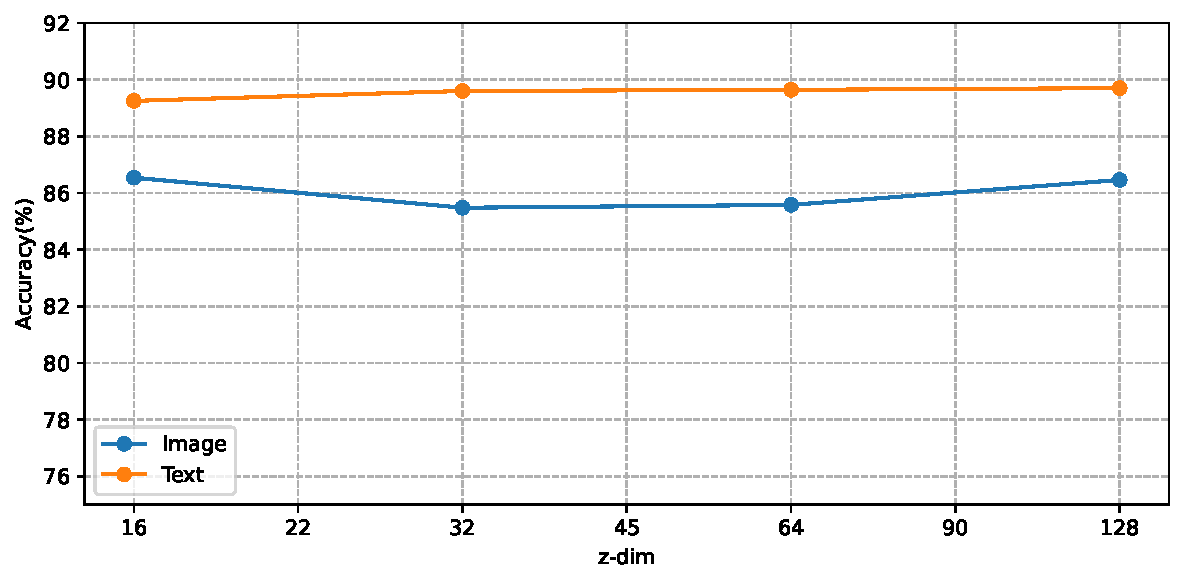
\includegraphics[width=\textwidth]{figs/mega/mega_z.pdf}
\caption{z-dim}
\label{fig:mega_z}
\end{subfigure}
\hspace{0.05\textwidth}
\begin{subfigure}[b]{0.45\textwidth}
\centering
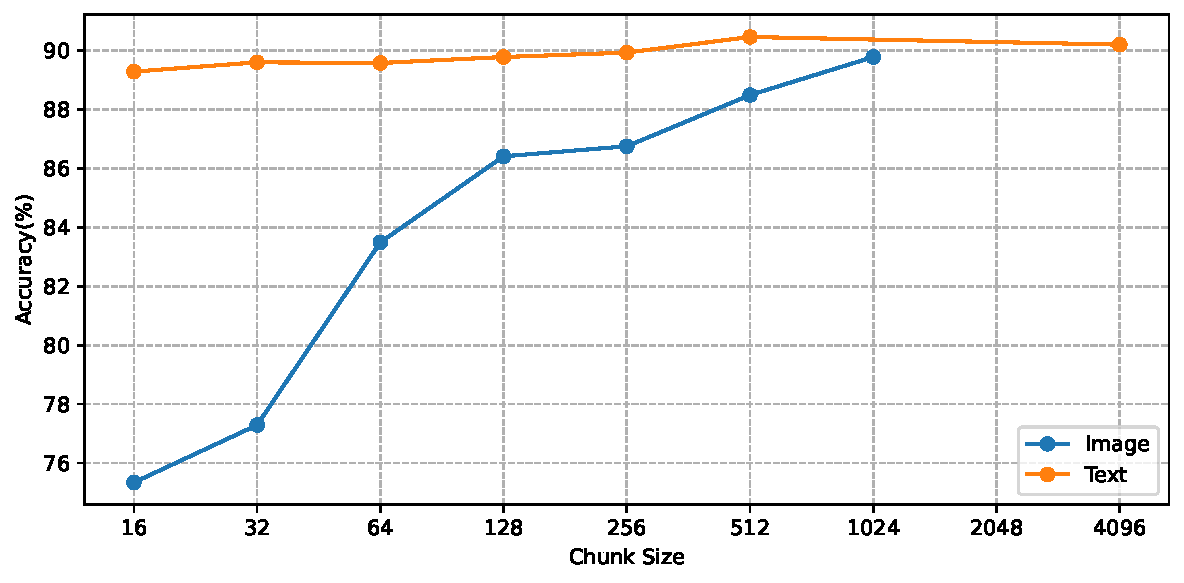
\includegraphics[width=\textwidth]{figs/mega/mega_chunk.pdf}
\caption{chunk size}
\label{fig:mega_chunk}
\end{subfigure}

\caption{MEGA 模型参数对性能的影响}
\label{fig:mega_param}
\end{figure}

\subs{MEGA 方法参数}
对于 MEGA 而言,其提升计算效率的关键在于使用 MEGA-chunk,并尽可能减小分块大小 $c$ 的值。然而过小的 $c$ 导致远距离相关的元素需要更为复杂的传递才能相互作用。这可能使得模型处理远距离信息的能力变弱。因此,我们选取了两个较为有代表性的任务:上下文长度为 4K 的 Text 作为长序列的典型任务,以及上下文长度为 1K 的 Image 作为复杂序列关系的典型任务,来探索部分 MEGA 参数对于建模能力的影响。

首先是MEGA 中序列的高效表征向量 z 的维度。选取维度为$2^4,2^5,2^6,2^7$(即实验中用到的最大值)分别进行训练和推理,结果如图 \ref{fig:mega_z} 所示。可见不同大小的 z 对模型的性能表现几乎没有影响。这很可能是因为 z 维度的特征在计算 Attention 时会被压缩为 1 维的注意力权重,因此即使 16 维的向量也已经携带了充分的信息。换言之,在 Attention计算过程中看似损失的位数可能已经被对z向量的投影过程所补偿。

接下来是 chunk 大小。选用 $c=2^4, 2^5,\cdots,2^{12}$ 分别训练并测量模型的建模效果,结果如图\ref{fig:mega_chunk}所示。实验发现对 Text 任务,跨越多个数量级的 chunk 大小并未对结果产生显著影响,而对于 Image 来说,准确率随 chunk 的增大显著增加。Text 任务中靠相临近的词产生关联即可较为准确的确定情感,此时信息传递效率就并非准确率的瓶颈。而对于 Image 来说,一维距离很远的点可能二维距离很近,因此过小的 chunk 大小显著限制了需要产生相关性的元素之间的相互作用。结合\ref{subsec:lra_perf}中 MEGA-128 在 ListOps 上表现不佳的观察,这很可能说明 MEGA-chunk 在元素具有复杂位置关联的任务上有较大的精度损失。

\s{总结}
    在本学期的“数值分析”课程项目中,我们探究了 CosFormer,LARA,SkyFormer 和 MEGA 这 4 种模型加速计算 Self-Attention 的原理,并实际测试了它们的建模能力,验证了它们在训练和推理过程中的加速效果。实验结果表明,以上 4 种 Self-Attention 的快速计算机制总体来说可以与普通的 Self-Attention 达到类似的长序列建模效果。虽然各有局限性,但它们在较长的序列上,都能较为显著地减少训练和推理过程中的显存开销和时间占用。


\microtypesetup{protrusion=false}
\printbibliography[heading=refheading]

\end{document}